% !TeX encoding = UTF-8

% 载入 SJTUThesis 模版
\documentclass[type=course,lang=en]{sjtuthesis}
% 选项
%   type=[doctor|master|bachelor|course],     % 可选(默认:doctor),论文类型
%   zihao=[-4|5],                             % 可选(研究生默认:-4,本科默认:5),正文字号大小
%   lang=[zh|en],                             % 可选(默认:zh),论文的主要语言
%   review,                                   % 可选(默认:关闭),盲审模式
%   [twoside|oneside]                         % 可选(默认:twoside),单双页模式

% 论文基本配置,加载宏包等全局配置
% !TEX root = ./main.tex

\sjtusetup{
  %
  %******************************
  % 注意:
  %   1. 配置里面不要出现空行
  %   2. 不需要的配置信息可以删除
  %******************************
  %
  % 信息录入
  %
  info = {%
    %
    % 标题
    %
    title           = {上海交通大学学位论文 \LaTeX{} 模板示例文档},
    title*          = {Linux Race-Averse Scheduler},
    %
    % 标题页标题
    %   可使用“\\”命令手动控制换行
    %
    % display-title   = {上海交通大学学位论文\\ \LaTeX{} 模板示例文档},
    % display-title*  = {A Sample Document \\ for \LaTeX-based SJTU Thesis Template},
    %
    % 页眉标题
    %
    % running-title   = {示例文档},
    % running-title*  = {Sample Document},
    %
    % 关键词
    %
    keywords        = {上海交大, 饮水思源, 爱国荣校},
    keywords*       = {Linux Scheduler, Memory Access Tracing, Race-Averse, Weighted Round Robin},
    %
    % 姓名
    %
    author          = {某\quad{}某},
    author*         = {Mo Mo},
    %
    % 指导教师
    %
    supervisor      = {某某教授},
    supervisor*     = {Prof. Mou Mou},
    %
    % 副指导教师
    %
    % assisupervisor  = {某某教授},
    % assisupervisor* = {Prof. Uom Uom},
    %
    % 学号
    %
    id              = {0010900990},
    %
    % 学位
    %   本科生不需要填写
    %
    degree          = {工学硕士},
    degree*         = {Master of Engineering},
    %
    % 专业
    %
    major           = {某某专业},
    major*          = {A Very Important Major},
    %
    % 所属院系
    %
    department      = {某某系},
    department*     = {Depart of XXX},
    %
    % 课程名称
    %   仅课程论文适用
    %
    course          = {某某课程},
    %
    % 答辩日期
    %   使用 ISO 格式 (yyyy-mm-dd);默认为当前时间
    %
    % date            = {2014-12-17},
    %
    % 资助基金
    %
    % fund  = {
    %           {国家 973 项目 (No. 2025CB000000)},
    %           {国家自然科学基金 (No. 81120250000)},
    %         },
    % fund* = {
    %           {National Basic Research Program of China (Grant No. 2025CB000000)},
    %           {National Natural Science Foundation of China (Grant No. 81120250000)},
    %         },
  },
  %
  % 风格设置
  %
  style = {%
    %
    % 本科论文页眉 logo 颜色 (red/blue/black)
    %
    % header-logo-color = black,
  },
  %
  % 名称设置
  %
  name = {
    % bib               = {References},
    % acknowledgements  = {谢\hspace{\ccwd}辞},
    % publications      = {攻读学位期间完成的论文},
  },
}

% 使用 BibLaTeX 处理参考文献
%   biblatex-gb7714-2015 常用选项
%     gbnamefmt=lowercase     姓名大小写由输入信息确定
%     gbpub=false             禁用出版信息缺失处理
\usepackage[backend=biber,style=gb7714-2015]{biblatex}
% 文献表字体
% \renewcommand{\bibfont}{\zihao{-5}}
% 文献表条目间的间距
\setlength{\bibitemsep}{0pt}
% 导入参考文献数据库
\addbibresource{bibdata/thesis.bib}

% 定义图片文件目录与扩展名
\graphicspath{{figures/}}
\DeclareGraphicsExtensions{.pdf,.eps,.png,.jpg,.jpeg}

% 确定浮动对象的位置,可以使用 [H],强制将浮动对象放到这里(可能效果很差)
% \usepackage{float}

% 固定宽度的表格
% \usepackage{tabularx}

% 使用三线表:toprule,midrule,bottomrule。
\usepackage{booktabs}

% 表格中支持跨行
\usepackage{multirow}

% 表格中数字按小数点对齐
\usepackage{dcolumn}
\newcolumntype{d}[1]{D{.}{.}{#1}}

% 使用长表格
\usepackage{longtable}

% 附带脚注的表格
\usepackage{threeparttable}

% 附带脚注的长表格
\usepackage{threeparttablex}

% 算法环境宏包
\usepackage[ruled,vlined,linesnumbered]{algorithm2e}
% \usepackage{algorithm, algorithmicx, algpseudocode}

% 代码环境宏包
\usepackage{listings}
\lstnewenvironment{codeblock}[1][]%
  {\lstset{style=lstStyleCode,#1}}{}

% 物理科学和技术中使用的数学符号,定义了 \qty 命令,与 siunitx 3.0 有冲突
% \usepackage{physics}

% 直立体数学符号
\newcommand{\dd}{\mathop{}\!\mathrm{d}}
\newcommand{\ee}{\mathrm{e}}
\newcommand{\ii}{\mathrm{i}}
\newcommand{\jj}{\mathrm{j}}

% 国际单位制宏包
\usepackage{siunitx}[=v2]

% 定理环境宏包
\usepackage{ntheorem}
% \usepackage{amsthm}

% 绘图宏包
\usepackage{tikz}
\usetikzlibrary{shapes.geometric, arrows}

% 一些文档中用到的 logo
\usepackage{hologo}
\newcommand{\XeTeX}{\hologo{XeTeX}}
\newcommand{\BibLaTeX}{\textsc{Bib}\LaTeX}

% 借用 ltxdoc 里面的几个命令方便写文档
\DeclareRobustCommand\cs[1]{\texttt{\char`\\#1}}
\providecommand\pkg[1]{{\sffamily#1}}

% 自定义命令

% E-mail
\newcommand{\email}[1]{\href{mailto:#1}{\texttt{#1}}}

% hyperref 宏包在最后调用
\usepackage{hyperref}

\usepackage{svg}

% 自动引用题注更正为中文
\def\equationautorefname{式}
\def\footnoteautorefname{脚注}
\def\itemautorefname{项}
\def\figureautorefname{图}
\def\tableautorefname{表}
\def\partautorefname{篇}
\def\appendixautorefname{附录}
\def\chapterautorefname{章}
\def\sectionautorefname{节}
\def\subsectionautorefname{小节}
\def\subsubsectionautorefname{小节}
\def\paragraphautorefname{段落}
\def\subparagraphautorefname{子段落}
\def\FancyVerbLineautorefname{行}
\def\theoremautorefname{定理}


\begin{document}

%TC:ignore

% 标题页
% \maketitle
\begin{titlepage}
   \begin{center}
        \vspace*{4cm} % Adjust spacings to ensure the title page is generally filled with text

        \Huge{OS Project 2 Report} 

        \vspace{0.5cm}
        \LARGE{Linux Race-Averse Scheduler}
            
        \vspace{3 cm}
        \Large{}
       
        \vspace{0.25cm}
        \large{Ziqian Zhao 520021910171}
       
        \vspace{3 cm}
        \Large{May 10, 2022}
        
        \vspace{0.25 cm}
        \Large{}
       

       \vfill
    \end{center}
\end{titlepage}

% 原创性声明及使用授权书
% \copyrightpage
% 插入外置原创性声明及使用授权书
% \copyrightpage[scans/sample-copyright-old.pdf]

% 前置部分
\frontmatter

% 摘要
% !TEX root = ../main.tex

\begin{abstract*}
  In this project, we first implement a Memory Access Tracing (MAT) method to trace the number of times a given range of memory is written by a particular task. Then, based on the Memory Access Tracing, we design a Race-Averse Linux Process Scheduler (RAS), using a Weighted Round Robin style according to race probabilities of each task. Furthermore, we benchmark the performance of Linux native schedulers and our Race-Averse Scheduler. The results prove that RAS achieves higher throughput, shorter turnaround time and lower latency.
\end{abstract*}


% 目录
\tableofcontents
% 插图索引
% \listoffigures*
% 表格索引
% \listoftables*
% 算法索引
% \listofalgorithms*

% 符号对照表
% % !TEX root = ../main.tex

\begin{nomenclature*}
\label{chap:symb}

\begin{longtable}{rl}
  $\epsilon$  & 介电常数  \\  
  $\mu$       & 磁导率    \\
  $\epsilon$  & 介电常数  \\
  $\mu$       & 磁导率    \\
  $\epsilon$  & 介电常数  \\
  $\mu$       & 磁导率    \\
  $\epsilon$  & 介电常数  \\
  $\mu$       & 磁导率    \\
  $\epsilon$  & 介电常数  \\
  $\mu$       & 磁导率    \\
  $\epsilon$  & 介电常数  \\
  $\mu$       & 磁导率    \\
  $\epsilon$  & 介电常数  \\
  $\mu$       & 磁导率    \\
  $\epsilon$  & 介电常数  \\
  $\mu$       & 磁导率    \\
  $\epsilon$  & 介电常数  \\
  $\mu$       & 磁导率    \\
  $\epsilon$  & 介电常数  \\
  $\mu$       & 磁导率    \\
  $\epsilon$  & 介电常数  \\
  $\mu$       & 磁导率    \\
  $\epsilon$  & 介电常数  \\
  $\mu$       & 磁导率    \\
  $\epsilon$  & 介电常数  \\
  $\mu$       & 磁导率    \\
  $\epsilon$  & 介电常数  \\
  $\mu$       & 磁导率    \\
  $\epsilon$  & 介电常数  \\
  $\mu$       & 磁导率    \\
  $\epsilon$  & 介电常数  \\
  $\mu$       & 磁导率    \\
  $\epsilon$  & 介电常数  \\
  $\mu$       & 磁导率    \\
  $\epsilon$  & 介电常数  \\
  $\mu$       & 磁导率    \\
  $\epsilon$  & 介电常数  \\
  $\mu$       & 磁导率    \\
  $\epsilon$  & 介电常数  \\
  $\mu$       & 磁导率    \\
  $\epsilon$  & 介电常数  \\
  $\mu$       & 磁导率    \\
  $\epsilon$  & 介电常数  \\
  $\mu$       & 磁导率    \\
  $\epsilon$  & 介电常数  \\
  $\mu$       & 磁导率    \\
  $\epsilon$  & 介电常数  \\
  $\mu$       & 磁导率    \\
  $\epsilon$  & 介电常数  \\
  $\mu$       & 磁导率    \\
  $\epsilon$  & 介电常数  \\
  $\mu$       & 磁导率    \\
  $\epsilon$  & 介电常数  \\
  $\mu$       & 磁导率    \\
\end{longtable}

\end{nomenclature*}


%TC:endignore

% 主体部分
\mainmatter

% 正文内容
% !TEX root = ../main.tex

\chapter{Memory Access Tracing}

\section{MAT Introduction}

In Linux, tracing memory access for tasks\footnote{In Linux Scheduler, processes and threads are often treated equally, so here we don't make clear distinction, and refer to both processes and threads as tasks.} is useful. Although the hardware uses a R bit and a M bit to track if a page has been referenced or modified, it does not maintain access frequency for each task. Therefore, we try to propose a per task memory access tracing method, which can trace the number of times a given range of memory is written by a particular task. Based on the tracing mechanism, we can use these tracing data to calculate the race probabilities between different tasks.

\section{MAT Design}

To tracing the writes of a given range of memory, we can take full advantage of the Page Fault mechanism. Firstly, invoke linux system call \textit{mprotect} on given range of memory before any writes to set the memory as Read-Only. The system call \textit{mprotect} changes the access protections for the calling task's memory pages containing any part of the given address range. If the calling task tries to access memory in a manner that violates the protections, then the kernel generates a SIGSEGV signal for the task\cite{mprotect}. Now, if we try to write to the protected memory, the kernel will send us a SIGSEGV signal. Secondly, after capturing the signal in user space, we can customize the method to deal with it. We call it the SIGSEGV handler. In the handler, we just simply invoke the \textit{mprotect} again, but this time we set the memory as Read-Write. Then we can write to the memory normally. Thirdly, in the kernel space, on the path that the kernel generates the SIGSEGV signal due to access permission error, we can perceive that in the user space a write was performing. Thus, memory access tracing is achieved.

\begin{figure}[!htp]
  \centering
  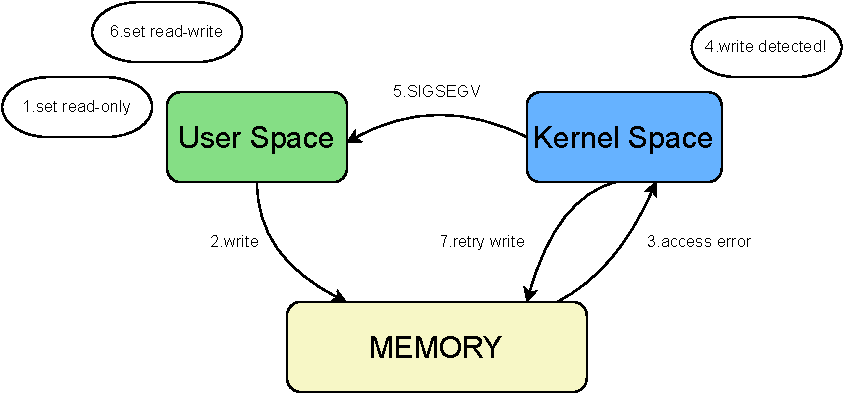
\includegraphics[width=12cm]{figures/memaccess.drawio.pdf}
  \caption{Memory Access Tracing Procedure}
\end{figure}

After the analysis above, we can find that to detect and record memory writes, we need to do some modification on the path that the kernel sends the SIGSEGV signal. If a SIGSEGV is to be generated and we are tracing the task, the kernel would add one to the write counts of the task.

\section{MAT Implementation}

To apply the memory access tracing to linux kernel, we implement three system calls. Load the three modules into the kernel, and then we can use these system calls to start tracing, stop tracing, and getting the tracing results:

\begin{itemize}
    \item \textbf{\textit{sys\_start\_trace(pid\_t pid)}}: tell the kernel to start tracing memory writes of the given pid.
    \item \textbf{\textit{sys\_stop\_trace(pid\_t pid)}}: tell the kernel to stop tracing memory writes of the given pid.
    \item \textbf{\textit{sys\_get\_trace(pid\_t pid, int *wcounts)}}: get the memory writes times of the given pid.
\end{itemize}

Besides, we add some variables to the \textit{task\_struct}\footnote{\textit{task\_struct} is a data structure in linux kernel. It records the information of a process.} to record the tracing states of the task. Finally, we add some code to the kernel on the path to send SIGSEGV. These code segments will update the write counts if we are tracing the running task.

\subsection{Task Struct}

We add a integer variable \textit{wcounts} to record the write times and a boolean variable \textit{trace\_flag} to determine when to start tracing:

\begin{codeblock}[language=C]
// include/linux/sched.h
struct task_struct {
	... 
	int wcounts; // record the write times	
	int trace_flag;	// 0 not tracing, 1 tracing
  ...
};
\end{codeblock}

\subsection{Update Write Count}

In the kernel source code of the page fault process, we add some code to update the write counts if we are tracing the task:

\begin{codeblock}[language=C]
// arch/arm/mm/fault.c
static int __kprobes
do_page_fault(unsigned long addr, unsigned int fsr, struct pt_regs *regs)
{
    ...
    if (fault & VM_FAULT_SIGBUS) {
		...
	  } else {
	    ... 
		  if (tsk->trace_flag) // SIGSEGV! If tracing, add one to task wcounts	
		  	tsk->wcounts++;
	  }
	  ...
}
\end{codeblock}

\subsection{System Calls}

In \textit{sys\_start\_trace}, we set the \textit{trace\_flag} of the task corresponding to the given pid to 1. If we have already been tracing the task, do nothing and return \textit{-EINVAL}:

\begin{codeblock}[language=C]
static int sys_start_trace(pid_t pid)
{
    struct task_struct *task;
    task = get_pid_task(find_get_pid(pid), PIDTYPE_PID); // get task by pid
    if (!task || task->trace_flag == 1)
        return -EINVAL;
    task->trace_flag = 1; // start tracing
    task->wcounts = 0;
    return 0;
}
\end{codeblock}

In \textit{sys\_stop\_trace}, we set the \textit{trace\_flag} to 0, and reset the \textit{wcounts} to 0. If we haven't traced the task yet, return \textit{-EINVAL}:

\begin{codeblock}[language=C]
static int sys_stop_trace(pid_t pid)
{
    struct task_struct *task;
    task = get_pid_task(find_get_pid(_pid), PIDTYPE_PID); // get task by pid
    if (!task || task->trace_flag == 0)
        return -EINVAL;
    task->trace_flag = 0; // stop tracing
    task->wcounts = 0;
    return 0;
}
\end{codeblock}

In \textit{sys\_get\_trace}, we get the task's \textit{wcounts}. If we haven't traced the task yet, return \textit{-EINVAL}:

\begin{codeblock}[language=C]
static int sys_get_trace(pid_t _pid, int *wcounts)
{
    struct task_struct *task;
    task = get_pid_task(find_get_pid(_pid), PIDTYPE_PID); // get task by pid
    if (!task || task->trace_flag == 0)
        return -EINVAL;
    *wcounts = task->wcounts; // get the wcounts
    return 0;
}
\end{codeblock}

\section{MAT Test}

We have written a test program to test three system calls and memory access tracing we implement. The test results are shown as following:

\begin{figure}[!htp]
\begin{minipage}{0.48\textwidth}
  \centering
  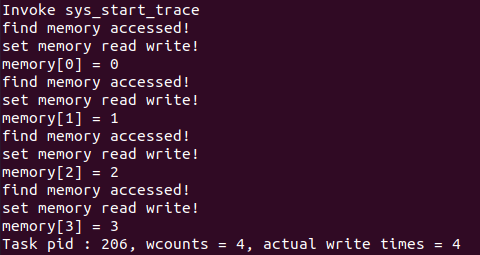
\includegraphics[height=3.8cm]{figures/mattest1.png}
  \caption{Start Tracing Test}
  \label{fig:memtest1}
\end{minipage}\hfill
\begin{minipage}{0.48\textwidth}
  \centering
  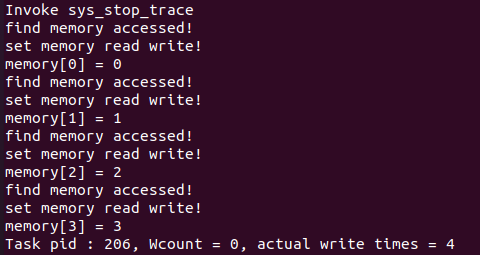
\includegraphics[height=3.8cm]{figures/mattest2.png}
  \caption{Stop Tracing Test}
  \label{fig:memtest2}
\end{minipage}
\end{figure}

In Figure~\ref{fig:memtest1} we can see that after we invoke \textit{sys\_start\_trace}, the memory access tracer can record the write times correctly. In Figure~\ref{fig:memtest2} we can see that after we invoke \textit{sys\_stop\_trace}, the kernel would stop tracing the task's memory accesses. Thus, we successfully implement the memory access tracing.

\section{MAT Conclusion}

In this project, we implemented the Memory Access Tracing and got the correct test results. Using the tracing data, we can further compute the race probabilities between different tasks. This can help us to accomplish the Race-Averse Scheduler.

However, there still exist some imperfections in our implementation. First, the tracing can not be done only by kernel. We have to use \textit{mprotect} to set protection for the memory before any write in user space. Can we set protection automatically in kernel space? If we achieve this, we can trace the memory access only by invoking \textit{sys\_start\_trace}, and perform writes without additional explicit protection in user space, which is apparently more reasonable and elegant. Second, because we borrow the page fault handler to detect the writes in kernel space, every write associated with the tracing memory will result in a page fault. Is it an acceptable overhead? If it significantly affects the write performance, we have to re-evaluate its value.

% !TEX root = ../main.tex

\chapter{Race-Averse Scheduler}

\section{RAS Introduction}

CPU scheduling is the basis of multiprogrammed operating systems. By switching the CPU among tasks, the operating system can make the computer more productive. In a single-processor system, only one task can run at a time. Others must wait until the CPU is free and can be rescheduled\cite{schedintro}. Through frequently scheduling and context switch, tasks can run in a concurrent manner. The role of the Linux scheduler is to select the next task to run and distribute the running time.

Linux implements several kinds of schedulers for different scheduling situation. For example, Linux has RT Scheduler for real-time tasks, CFS Scheduler for normal tasks and IDLE Scheduler for tasks with least importance. When these schedulers pick a task, they take a variety of factors into account. However, the likelihood that a task may race with other currently running tasks is not considered. Therefore, we propose a Race-Averse Scheduling (RAS) algorithm. The scheduling is a Weighted Round Robin style scheduling according to race probabilities of each running task.

\section{RAS Design}

\subsection{How RAS works}

First we will introduce the Weighted Round Robin scheduling. Round Robin scheduling treats all tasks equally. It distribute the same \textit{timeslice}\footnote{A concept in Linux Scheduling. Refers to a period of time for the task to run. Usually 10ms\textasciitilde100ms.} to every picked task. When a task runs out of its timeslice, it would yield the execution by its self, and be put back on the end of the \textit{run queue}\footnote{A concept in Linux Scheduling. Every task which is ready but not running will be waiting in the run queue for being picked to run.}. 

\begin{figure}[!htp]
  \centering
  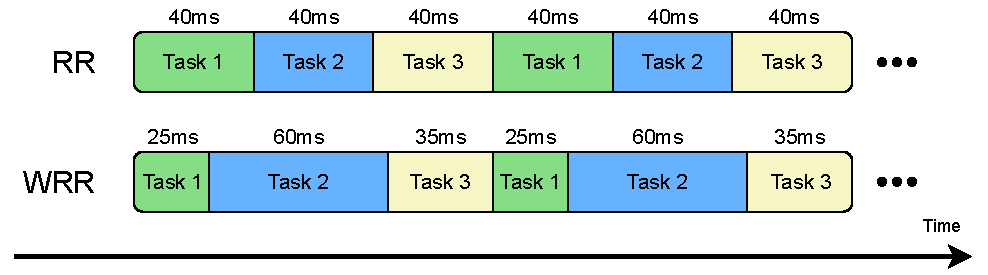
\includegraphics[width=12cm]{figures/wrr.drawio.pdf}
  \caption{Round Robin \& Weighted Round Robin}
\end{figure}

However, there are some situations where it is desirable to give some tasks preference over the others. That is, distributing longer timeslice to some tasks. Weighted Round Robin actually does this. The only difference between Round Robin and Weighted Round Robin is that Weighted Round Robin will assign a weight to each task, and tasks with higher weights will be given longer timeslice to run.

Obviously, in Race-Averse Scheduler, the weights are determined by the race probabilities. In our design, the race probability of a task is represented as an integer in the range of [0, 10). The higher the integer is, the more likely that the task may race with others. For CPU, it is rational to give preference to the tasks with lower race probabilities. That is exactly what the Race-Averse means. Therefore, tasks with lower race probabilities will be assigned with higher weights, which is, with longer timeslice to run. 

With the assistance of the Memory Access Tracing we implemented before, we can quantify the race probabilities between different running tasks. To simplify the situation, we assume that a large enough number of tasks are in scheduling, and they may compete at a given range of virtual addresses. Thus, the race probability of a certain task is proportional to its frequency of accessing the given range of virtual addresses. We can use the following equation to calculate the race probability:

\begin{equation}
    race\_prob_i = 10\times\frac{wcounts_i}{\sum_{i}wcounts_i}
\end{equation}

We set the maximum timeslice of the Race-Averse Scheduler to 100ms and the minimum timeslice to 10ms. And we can inversely map the race probabilities from 0 to 9 into the timeslice from 100ms to 10ms:


\begin{equation}
\begin{aligned}
    timeslice &= \frac{max\_timeslice-min\_timeslice}{0-9}\times race\_prob+max\_timeslice\\
    &= -10ms\times race\_prob + max\_timeslice
\end{aligned}
\end{equation}

When a task runs out of its timeslice, the RAS will compute the sum of \textit{wcounts} of the tasks in RAS run queue, and further calculate its race probability. Then assign a new timeslice according to its race probability, and put the task back to the end of the run queue. We should notice that the weight of a task can be changed dynamically, due to the newly coming tasks, completed tasks and some other reasons. Therefore, we have to re-compute the race probability every time the task needs to be assigned with new timeslice.

\subsection{Into Linux Kernal}

Now we are familiar with how the Race-Averse Scheduler works. Next, we will look into the Linux kernel and introduce how to embed the Race-Averse Scheduler into the kernel.

There are many ready tasks waiting for running in kernel. To manage these tasks, the kernel maintains a \textit{Run Queue} of these tasks. Besides, we call the task that the CPU is running \textit{Current Task}. To switch different tasks to Current Task, first the kernel should set the \textit{Need Resched} flag to Current Task, and second the kernel should check the Need Resched flag at a proper time. If Current Task needs to be rescheduled, the kernel calls \textit{Schedule} function to perform a context switch. The proper time actually refers to the time when CPU is interrupted by the ticker timer and etc. 

The Schedule function picking the next task needs the help of \textit{Scheduling Class}. Linux uses Scheduling Class to implement different scheduling algorithms. Here we take \textit{rt\_sched\_class}\footnote{\textit{rt\_sched\_class} implements FIFO and RR scheduling algorithms.}, \textit{cfs\_sched\_class}\footnote{\textit{cfs\_sched\_class} implements Completely Fair Scheduling algorithm.}, \textit{idle\_sched\_class}\footnote{\textit{idle\_sched\_class} implements IDLE scheduling algorithm.} and our \textit{ras\_sched\_class} as example. These classes are linked together through a linked list. When Schedule function wants to pick the next task, it will iterate through the schedule classes linked list and try to get a task from their own run queues. Once it gets a valid task, it would return directly and set the task as Current Task. So it is easy to see that every schedule class has different priorities. The head class of the linked list has higher priority than the tail class. Only when the former class doesn't have any task in run queue, the current class can pick its task in its run queue to return. Therefore, if we make different queue arrangement rules for different schedule classes, the tasks can be scheduled with different scheduling algorithms. For example, the run queue of \textit{rt\_sched\_class} contains multi priorities queues, and the run queue of \textit{cfs\_sched\_class} is a Red-Black Tree. From our previous discussion, we can learn that the run queue of RAS is a simple single queue.

\begin{figure}[!htp]
  \centering
  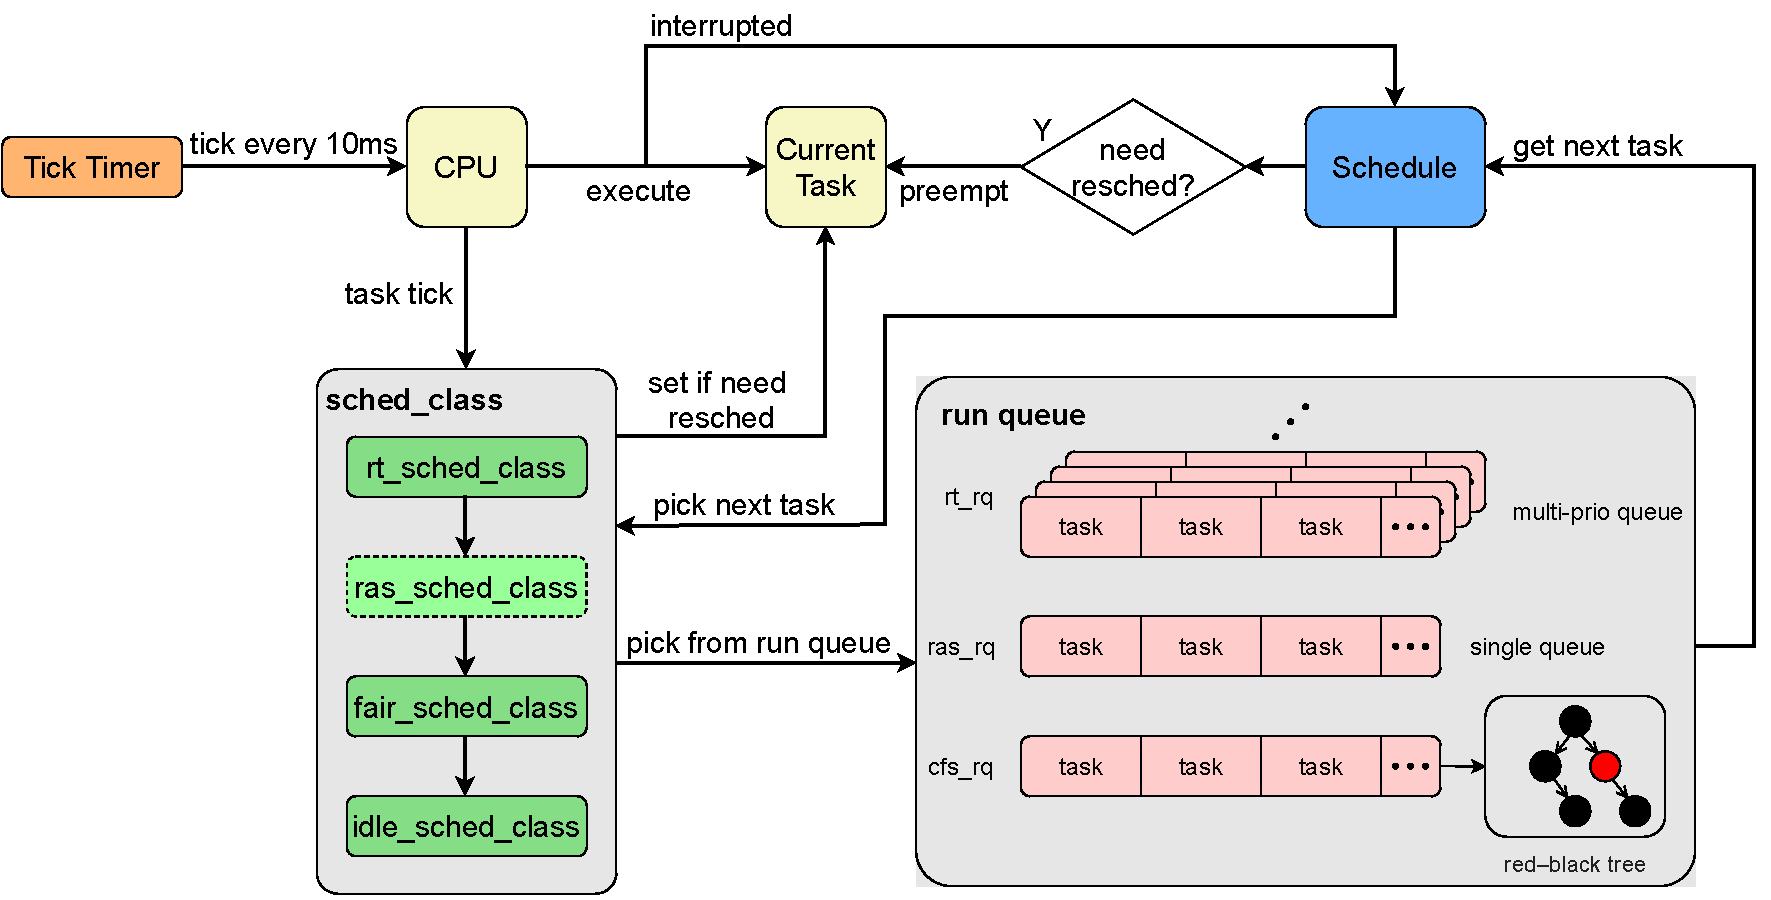
\includegraphics[width=14cm]{figures/scheduler.drawio.pdf}
  \caption{Linux Scheduling Procedure}
\end{figure}

Therefore, what we really need to implement is a new schedule class, \textit{ras\_sched\_class}.

\section{RAS Implementation}

The Scheduler Class has the following structure:

\begin{codeblock}[language=C]
// include/linux/sched.h
struct sched_class {
	const struct sched_class *next;
	void (*enqueue_task) (struct rq *rq, struct task_struct *p, int flags);
	void (*dequeue_task) (struct rq *rq, struct task_struct *p, int flags);
	struct task_struct* (*pick_next_task) (struct rq *rq);
	void (*task_tick) (struct rq *rq, struct task_struct *p, int queued);
	...
};
\end{codeblock}

All the scheduler classes should implement these functions. Their roles are closely related to the scheduling procedure of Linux Scheduler introduced above.

\begin{itemize}
    \item \textbf{\textit{next}}: points to the next scheduler class in the linked list. In our design, the next scheduler of RAS is Fair Scheduler, and the former scheduler of RAS is RT Scheduler.
    \item \textbf{\textit{enqueue\_task}}: enqueue a task into the run queue. 
    \item \textbf{\textit{dequeue\_task}}: dequeue a task from the run queue.
    \item \textbf{\textit{pick\_next\_task}}: pick a task from the run queue to be the next Current Task.
    \item \textbf{\textit{task\_tick}}: invoked when the tick timer ticks. Update some variables.
\end{itemize}

These four functions are the most important functions that we should implement for our Race-Averse Scheduler. Before implement these functions, we will define some structures associated with RAS.

\begin{figure}[!htp]
  \centering
  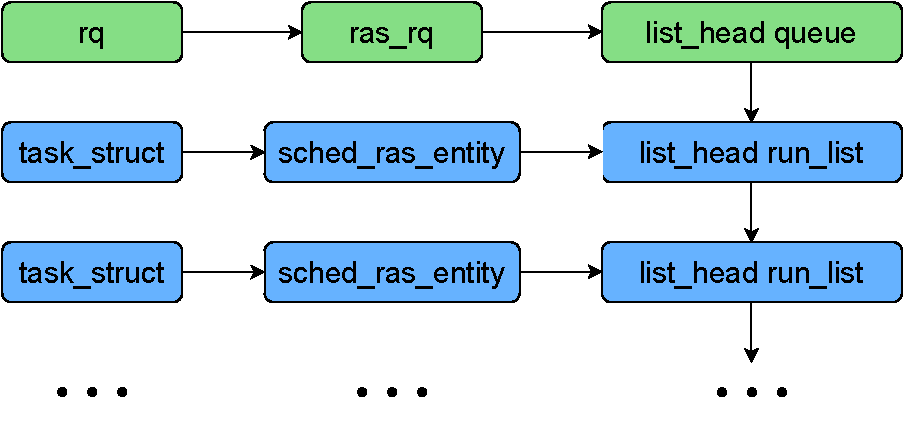
\includegraphics[width=11cm]{figures/structures.drawio.pdf}
  \caption{RAS Structures}
\end{figure}

\subsection{Structure ras\_rq}

Structure \textit{ras\_rq} is the implementation of the run queue of RAS. 

\begin{codeblock}[language=C]
// kernel/sched/sched.h
struct ras_rq 
{
	struct list_head queue;
	unsigned long ras_nr_running;
};
\end{codeblock}

\begin{itemize}
    \item \textbf{\textit{queue}}: the head of the RAS run queue linked list.
    \item \textbf{\textit{ras\_nr\_running}}: the number of tasks in RAS run queue.
\end{itemize}

\subsection{Structure sched\_ras\_entity}

Structure \textit{sched\_ras\_entity} represents an entity which can be scheduled by RAS, in other words, a task with the RAS scheduling strategy. Therefore, we should add a \textit{sched\_ras\_entity} variable in the \textit{task\_struct}.

\begin{codeblock}[language=C]
// include/linux/sched.h
struct sched_ras_entity 
{
	struct list_head run_list;
	unsigned int time_slice;
	unsigned int total_timeslice;
};
\end{codeblock}

\begin{itemize}
    \item \textbf{\textit{run\_list}}: the node in the RAS run queue linked list.
    \item \textbf{\textit{time\_slice}}: the timeslice left to run.
    \item \textbf{\textit{total\_timeslice}}: the timeslice allocated in this round.
\end{itemize}

With these structures defined, we can implement our RAS functions.

\subsection{Function enqueue\_task\_ras}

When a new task with RAS scheduling strategy comes into the kernel, or a task was switched from other scheduling strategy to RAS, the kernel will invoke \textit{enqueue\_task\_ras} to put the task into the RAS run queue.

\begin{codeblock}[language=C]
// kernel/sched/ras.c
static void
enqueue_task_ras(struct rq *rq, struct task_struct *p, int flags)
{
	struct sched_ras_entity *ras_se = &p->ras;
	struct ras_rq *ras_rq = &rq->ras;
	struct list_head *queue = &ras_rq->queue;
	list_add_tail(&ras_se->run_list, queue);
	ras_rq->ras_nr_running++;
	inc_nr_running(rq);
}
\end{codeblock}

We add the \textit{sched\_ras\_entity} to the tail of RAS run queue, and increase the count of running tasks.

\subsection{Function dequeue\_task\_ras}

When a task with RAS scheduling strategy finishes its job, or a task was switched from RAS to other scheduling strategy, the kernel will invoke \textit{dequeue\_task\_ras} to remove the task from the RAS run queue.

\begin{codeblock}[language=C]
// kernel/sched/ras.c
static void
dequeue_task_ras(struct rq *rq, struct task_struct *p, int flags)
{
	struct sched_ras_entity *ras_se = &p->ras;
	struct ras_rq *ras_rq = &rq->ras;
	list_del_init(&ras_se->run_list);
	ras_rq->ras_nr_running--;
	dec_nr_running(rq);
}
\end{codeblock}

We delete the \textit{sched\_ras\_entity} from RAS run queue, and decrease the count of running tasks.

\subsection{Function pick\_next\_task\_ras}

When the Scheduler function in the kernel wants to pick a task from the RAS run queue, \textit{pick\_next\_task\_ras} function will be called. It returns a task in the RAS run queue if there was.

\begin{codeblock}[language=C]
// kernel/sched/ras.c
static struct task_struct *
pick_next_task_ras(struct rq *rq)
{
	struct sched_ras_entity *ras_se;
	struct task_struct *p;
	struct ras_rq *ras_rq = &rq->ras;
	if (!ras_rq->ras_nr_running){
	  // No task in run queue, return null.
		return NULL;
	}
	struct list_head *queue = &ras_rq->queue;
	ras_se = list_entry(queue->next, struct sched_ras_entity, run_list);
	p = ras_task_of(ras_se);
	return p;
}
\end{codeblock}

The \textit{pick\_next\_task\_ras} function will select the head node of the run queue linked list to return. And if there is no task in run queue, it will return null.

\subsection{Function task\_tick\_ras}

The \textit{task\_tick\_ras} function is the most vital function for implementing Race-Averse Scheduler. In this function, we will compute the race probability of a task and dynamically allocate the task with some timeslice according to its race probability with other running tasks.

\begin{codeblock}[language=C]
// kernel/sched/ras.c
static void
task_tick_ras(struct rq *rq, struct task_struct *task, int queued)
{
	struct sched_ras_entity *ras_se = &task->ras;
	struct ras_rq *ras_rq = &rq->ras;
	if (task->policy != SCHED_RAS)
		return;		
	if (--task->ras.time_slice)
		return;
	if (ras_rq->ras_nr_running == 1){
		// No race. Set MAX timeslice to avoid frequently schedule.
		task->ras.time_slice = RAS_MAX_TIMESLICE;
		task->ras.total_timeslice = RAS_MAX_TIMESLICE;
	} else {
		// Calculate race probability.
		int wcounts = task->wcounts;
		struct list_head *p;
		struct sched_ras_entity *ras_se_tmp;
		struct task_struct *t;
		struct list_head *queue;
		queue = &ras_rq->queue;
		int sum = 0;
		int task_cnt = 0;
		list_for_each(p, queue)
		{
			ras_se_tmp = list_entry(p, struct sched_ras_entity, run_list);
			t = ras_task_of(ras_se_tmp);
			sum += t->wcounts;
			task_cnt++;
		}
		if (sum == 0 || sum == wcounts) {
			// not tracing or no memory write
			task->ras.time_slice = RAS_MAX_TIMESLICE;
			task->ras.total_timeslice = RAS_MAX_TIMESLICE;
		} else {
			int race_prob = wcounts * 10 / sum;
			unsigned int timeslice = -1*race_prob + RAS_MAX_TIMESLICE;
			task->ras.time_slice = timeslice;
			task->ras.total_timeslice = timeslice;
		}
	}
	
	// Requeue to the end of queue if we are NOT the only element on the queue.
	if (ras_se->run_list.prev != ras_se->run_list.next){
        requeue_task_ras(rq, task, 0);
        set_tsk_need_resched(task);
    }
}
\end{codeblock}

The \textit{task\_tick\_ras} function will be invoked every time the tick timer ticks. The tick timer ticks every 10ms. If the task has timeslice left, the function reduces its timeslice by one. If the task has no timeslice left, it indicates that the task should yield the CPU and be re-queued back to the tail of the run queue. Before the task is re-queued, it will be allocated with a new timeslice. If the task isn't being traced by Memory Access Tracer, or there is no memory write or task race, it will be allocated with the maximum timeslice. Otherwise, we iterate the tasks in the run queue and compute the race probability of the current task. Then allocate the timeslice according to its race probability.

\subsection{Some other functions}

With the four functions mentioned before, we can archive the basic operations of Race-Averse Scheduler. But we still need some other functions to implement the whole operations of RAS.

\begin{enumerate}
    \item \textit{\textbf{yield\_task\_ras}}: when the task wants to yield the CPU, this function will be called.
    \begin{codeblock}[language=C]
static void
yield_task_ras(struct rq *rq)
{
    requeue_task_ras(rq, rq->curr, 0);
}
    \end{codeblock}
    \item \textit{\textbf{update\_curr\_ras}}: update some statistical information of CPU and tasks.
    \begin{codeblock}[language=C]
static void update_curr_ras(struct rq *rq)
{
    struct task_struct *curr = rq->curr;
    struct sched_ras_entity *ras_se = &curr->ras;
    struct ras_rq *ras_rq = &rq->ras;
    u64 delta_exec;
    if (curr->sched_class != &ras_sched_class)
        return;
    delta_exec = rq->clock_task - curr->se.exec_start;
    if (unlikely((s64)delta_exec < 0))
        delta_exec = 0;
    schedstat_set(curr->se.statistics.exec_max,
	    		  max(curr->se.statistics.exec_max, delta_exec));
    curr->se.sum_exec_runtime += delta_exec;
    curr->se.exec_start = rq->clock_task;
}
    \end{codeblock}
    \item \textit{\textbf{put\_prev\_task\_ras}}: called before another task replaces the current task. For some statistical information.
    \begin{codeblock}[language=C]
static void
put_prev_task_ras(struct rq *rq, struct task_struct *p)
{
   	update_curr_ras(rq);
}
    \end{codeblock}
    \item \textit{\textbf{set\_curr\_task\_ras}}: called when the scheduling policy of the current task changes to RAS. For some statistical information.
    \begin{codeblock}[language=C]
static void
set_curr_task_ras(struct rq *rq)
{
	struct task_struct *p = rq->curr;
	p->se.exec_start = rq->clock_task;
}
    \end{codeblock}
    \item \textit{\textbf{get\_rr\_interval\_ras}}: return the total timeslice allocated before. For system calls.
    \begin{codeblock}[language=C]
static unsigned int
get_rr_interval_ras(struct rq *rq, struct task_struct *task)
{
	if (task->policy == SCHED_RAS)
	{
		struct sched_ras_entity *ras_se = &task->ras;
		return ras_se->total_timeslice;
	}
	return 0;
}
    \end{codeblock}
\end{enumerate}

Besides these structures and functions, we also have to re-write some code in the kernel source code to apply RAS to the kernel. For example, declare some variables and add some branch conditions of RAS. Please refer to the source code for detailed modification.

\section{RAS Test}

In this section, we write some test programs to check that whether RAS works correctly.

\subsection{Switch Test}

First, we launch a infinite loop program and get its \textit{pid}. Second, we use another program to change its scheduling policy to RAS, and then try to change back. Output information:

\begin{figure}[!htp]
  \centering
  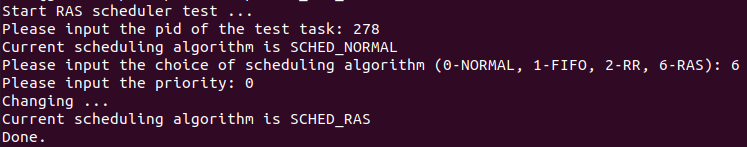
\includegraphics[width=12cm]{figures/basictest1.png}
  \caption{Change to RAS Policy}
  \label{fig:basictest1}
\end{figure}

\begin{figure}[!htp]
  \centering
  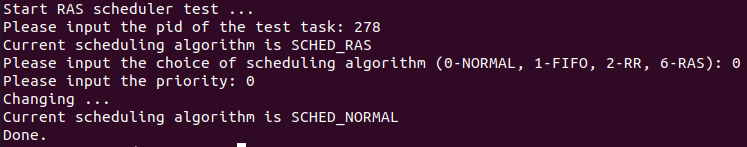
\includegraphics[width=12cm]{figures/basictest2.png}
  \caption{Change Back to NORMAL Policy}
  \label{fig:basictest2}
\end{figure}

In Figure~\ref{fig:basictest1} we can see that the task with pid 278 is successfully changed with the RAS policy. In Figure~\ref{fig:basictest2} we can see that it can also be changed back with the NORMAL policy. This proves that RAS is successfully embedded into Linux kernel.

\subsection{Multi-Tasks Test}

Now we write a test program to fork 10 child tasks and set their scheduling policy as RAS. Each task will write random times [128, 1024) to a given range of memory which is traced. Then we will check that RAS can whether correctly arrange their executions and allocate them with different timeslices according to their race probabilities. Output information is as following:

\begin{figure}[!htp]
  \centering
  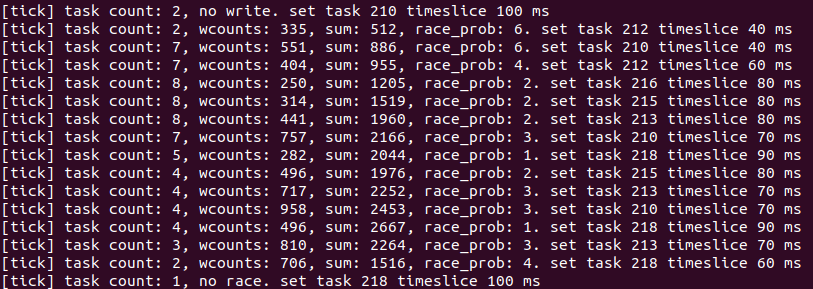
\includegraphics[width=13cm]{figures/multasktest1.png}
  \caption{RAS Multi Tasks Test Result}
  \label{fig:multitasktest}
\end{figure}

In Figure~\ref{fig:multitasktest} we can see that the RAS correctly scheduled these tasks in a weighted round robin style. When a task run out of its timeslice, it will be allocated with a new timeslice according to its race probability. Then it will be re-queued to the tail of the run queue. And RAS will pick the first task in the run queue as the next task to run.

These results prove that we successfully implemented the Race-Averse Scheduler.
% !TeX root = ../main.tex

\chapter{Benchmark}

\section{Benchmark Introduction}

We can benchmark a scheduler by many factors, for example, CPU utilization, throughput, turnaround time, latency, waiting time and etc. In this chapter, we will benchmark throughput, latency and turnaround time of SCHED\_NORMAL, SCHED\_FIFO, SCHED\_RR and SCHED\_RAS scheduling algorithms. 

\section{Benchmark Design}

First, we will explain the meaning of these test items in detail:
\begin{itemize}
    \item \textbf{throughput}: number of tasks that complete their execution per time unit.
    \item \textbf{latency}: time interval between the arrival of the task and the first execution of the task.
    \item \textbf{turnaround time}: time interval between the arrival of the task and the completion of the task.
\end{itemize}

We know that using Memory Access Tracing as the basis, RAS is write-sensitive. Thus, our benchmark program is I/O bound. The benchmark program will using \textit{mmap} system call to request a block of memory. We trace this memory's access using the tracer we implemented in Chapter One. Then benchmark program will fork a given number of child tasks to write random times into the memory. The four scheduling policies will be used in rotation under the same conditions.

\section{Benchmark Results}
\subsection{Throughput}

First, we benchmark the total running time of different scheduling policies with different task numbers. Each benchmark performs an average of 16368 writes per 10 tasks. The results are shown as following table:

\begin{table}[!hpt]
  \caption{Time Consumption of Each Benchmark (s)}
  \label{tab:firstone}
  \centering
  \begin{tabular}{*{6}{c}} \toprule
    \multirow{2}*{SCHED} & \multicolumn{5}{c}{Task Number} \\ \cmidrule(r){2-6}
    & 20 & 40 & 60 & 80 & 100 \\ 
    \midrule
    NORMAL & 22.259&30.568 &35.777 &41.616 & 50.145\\
    FIFO   & 7.441&15.152 &21.938 &28.863 & 37.169\\
    RR & 7.166&15.089 &21.776 &28.040 & 37.493\\
    RAS & 6.140&11.952 &17.358 &22.330 & 29.473\\
    \bottomrule
  \end{tabular}
\end{table}

It is apparent to see that RAS takes the least amount of time to complete the write tasks. FIFO and RR have nearly the same performance. NORMAL has the worst performance. Compared to FIFO and RR, RAS has about $20\%$ optimazation.

With the time consumption and task number of each scheduling algorithm, we can compute their throughput, number of tasks divided by time consumption. The results are as following chart:

\begin{figure}[!htp]
  \centering
  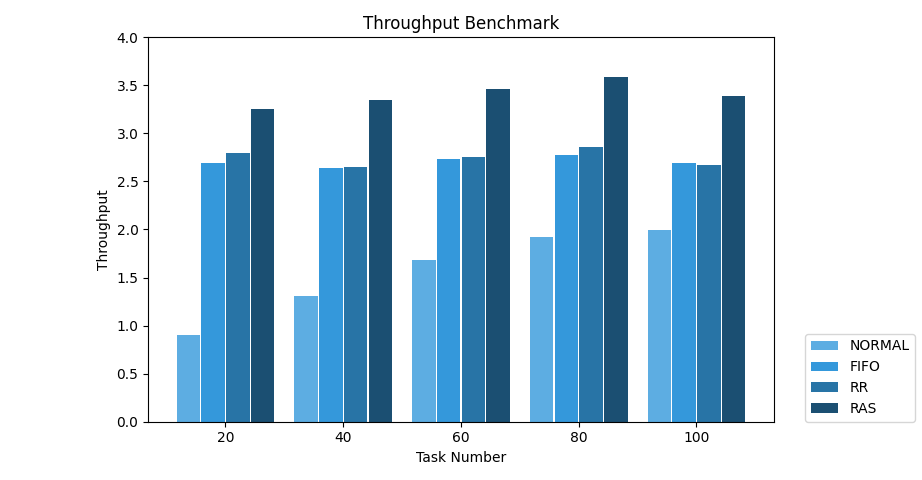
\includegraphics[width=13cm]{figures/throughput.png}
  \caption{Throughput Benchmark Result}
\end{figure}

In this chart we can see that RAS gets the highest throughput. For different task numbers, the throughput is about $3.4$ tasks per second. When the task number is too large, scheduling overhead may affect the throughput performance.

\subsection{Turnaround Time}

We record the fork time of a task and the completion time of it. And the turnaround time is their difference. A task will write minimum 16 times and maximum 8192 times. The results are as following chart:

\begin{figure}[!htp]
  \centering
  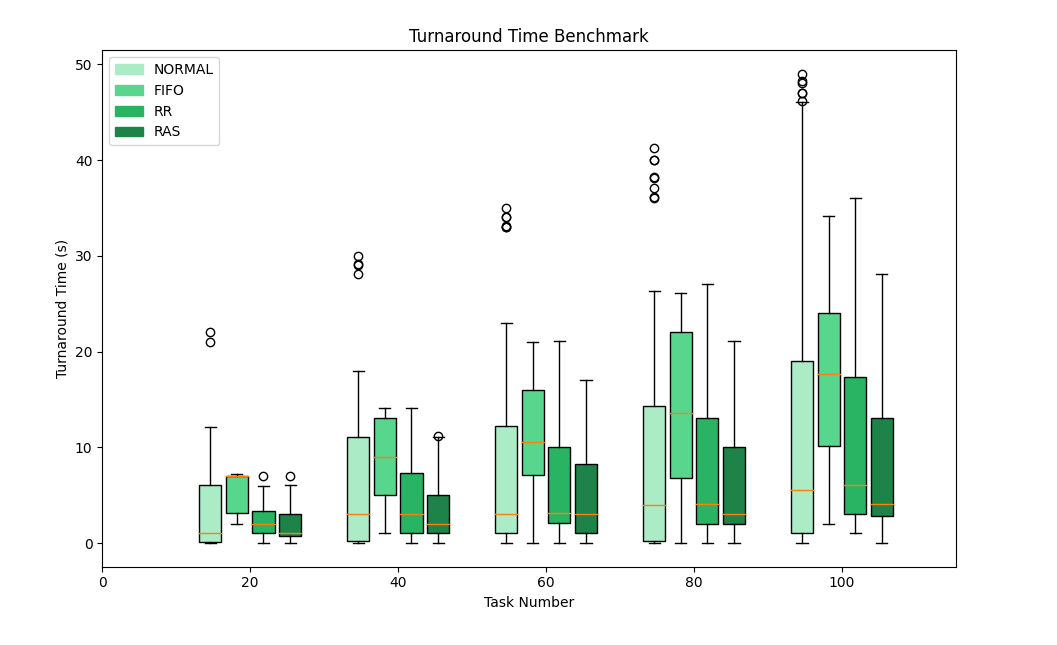
\includegraphics[width=13.5cm]{figures/turnaroundbox.png}
  \caption{Turnaround Time Benchmark Result}
  \label{fig:turnaroundbox}
\end{figure}

It is crystal clear that RAS gains the lowest average, the lowest median and the lowest upper boundary turnaround time. Besides, RAS also has the fewest outliers. It proves that among the four scheduler, RAS has the best and the most stable performance. Furthermore, we can notice that as the number of tasks increases, RAS will get better performance. And when task number is relatively low, RAS will achieve a similar performance to RR. This can be easily explained by the limited race situation when the number of tasks is small. Under these circumstances, the RAS will nearly allocate all the tasks with the maximum timeslice.

\subsection{Latency}

We use the difference between the fork time of a task and the first execution time to represent the latency. Also we choose 20, 40, 60, 80 and 100 task numbers and write minimum 16 times, maximum 8192 times. The results are as following chart:

\begin{figure}[!htp]
  \centering
  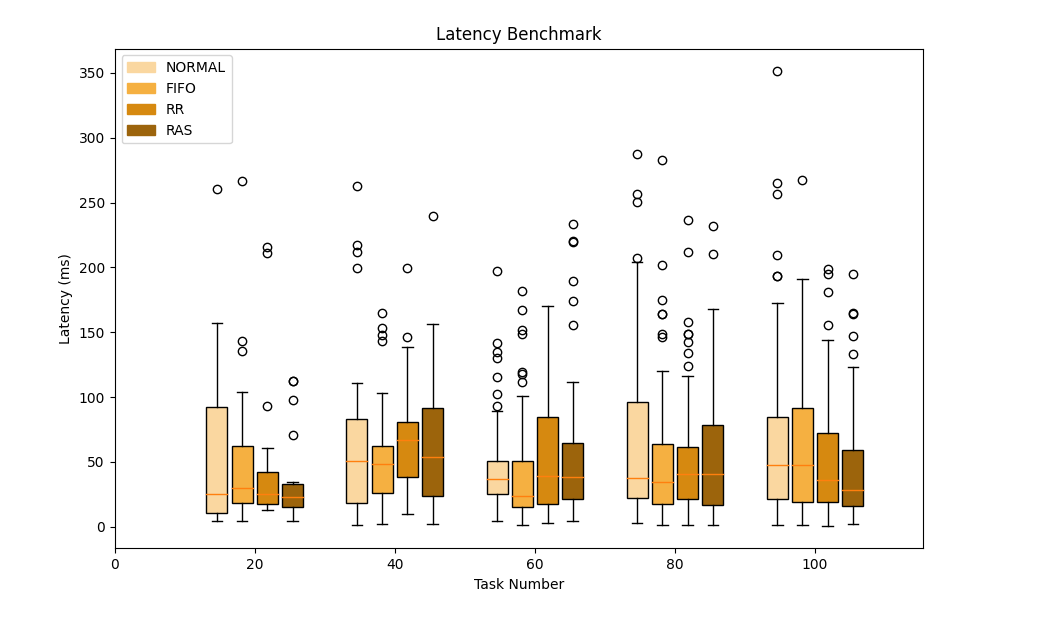
\includegraphics[width=13.5cm]{figures/latencybox.png}
  \caption{Latency Benchmark Result}
  \label{fig:turnaroundbox}
\end{figure}

In this chart we can find that RAS does not achieve great advantage in latency. The performances of RAS and RR are almost the same. The reason is that to reduce the overhead of context switch, we set the maximum timeslice (100ms, the same as RR timeslice) as the initial timeslice to RAS tasks. Therefore, when tasks first enter the kernel, they will be allocated with 100ms timeslice to run. That results in a larger latency for other tasks waiting for CPU. But compared to NORMAL and FIFO policies, RAS still gains optimization.



% !TEX root = ../main.tex

\begin{summary}
In this project, we first implemented the Memory Accessing Tracing method. Then, based on the tracer, we designed and implemented a new Linux scheduling algorithm RAS. Next, we successfully embedded it into Linux kernel, and proved that it can work correctly. Finally, we wrote several benchmark programs to test the performance of RAS and compared RAS with Linux native scheduling algorithms, NORMAL, FIFO and RR. The benchmark results shown that RAS has higher throughput, shorter \& more stable turnaround time and slightly lower latency.

Although the results are exciting, we still have to note that RAS has many limitations. For example, Memory Access Tracing can not be done completely in the kernel so far. Therefore, if we want to use RAS, we have to manually set protection for the specified memory again and again. Besides, RAS is only sensitive to write operation. So for CPU-bound tasks, RAS can not gain a better performance. We still need to make further improvements for RAS.

For me, this is my first time to read the Linux source code. That's a really challenge. But I learned a lot from it. This project has laid a foundation for me to explore the field of system in the future.
\end{summary}


%TC:ignore

% 参考文献
\printbibliography[heading=bibintoc]

% 附录
\appendix

% 附录中图表不加入索引
\captionsetup{list=no}

% 附录内容
% % !TEX root = ../main.tex

\chapter{Maxwell Equations}

选择二维情况,有如下的偏振矢量:
\begin{subequations}
  \begin{align}
    {\bf E} &= E_z(r, \theta) \hat{\bf z}, \\
    {\bf H} &= H_r(r, \theta) \hat{\bf r} + H_\theta(r, \theta) \hat{\bm\theta}.
  \end{align}
\end{subequations}
对上式求旋度:
\begin{subequations}
  \begin{align}
    \nabla \times {\bf E} &= \frac{1}{r} \frac{\partial E_z}{\partial\theta}
      \hat{\bf r} - \frac{\partial E_z}{\partial r} \hat{\bm\theta}, \\
    \nabla \times {\bf H} &= \left[\frac{1}{r} \frac{\partial}{\partial r}
      (r H_\theta) - \frac{1}{r} \frac{\partial H_r}{\partial\theta} \right]
      \hat{\bf z}.
  \end{align}
\end{subequations}
因为在柱坐标系下,$\overline{\overline\mu}$ 是对角的,所以 Maxwell 方程组中电场
$\bf E$ 的旋度:
\begin{subequations}
  \begin{align}
    & \nabla \times {\bf E} = \ii \omega {\bf B}, \\
    & \frac{1}{r} \frac{\partial E_z}{\partial\theta} \hat{\bf r} -
      \frac{\partial E_z}{\partial r}\hat{\bm\theta} = \ii \omega \mu_r H_r
      \hat{\bf r} + \ii \omega \mu_\theta H_\theta \hat{\bm\theta}.
  \end{align}
\end{subequations}
所以 $\bf H$ 的各个分量可以写为:
\begin{subequations}
  \begin{align}
    H_r &= \frac{1}{\ii \omega \mu_r} \frac{1}{r}
      \frac{\partial E_z}{\partial\theta}, \\
    H_\theta &= -\frac{1}{\ii \omega \mu_\theta}
      \frac{\partial E_z}{\partial r}.
  \end{align}
\end{subequations}
同样地,在柱坐标系下,$\overline{\overline\epsilon}$ 是对角的,所以 Maxwell 方程
组中磁场 $\bf H$ 的旋度:
\begin{subequations}
  \begin{align}
    & \nabla \times {\bf H} = -\ii \omega {\bf D}, \\
    & \left[\frac{1}{r} \frac{\partial}{\partial r}(r H_\theta) - \frac{1}{r}
      \frac{\partial H_r}{\partial\theta} \right] \hat{\bf z} = -\ii \omega
      {\overline{\overline\epsilon}} {\bf E} = -\ii \omega \epsilon_z E_z
      \hat{\bf z}, \\
    & \frac{1}{r} \frac{\partial}{\partial r}(r H_\theta) - \frac{1}{r}
      \frac{\partial H_r}{\partial\theta} = -\ii \omega \epsilon_z E_z.
  \end{align}
\end{subequations}
由此我们可以得到关于 $E_z$ 的波函数方程:
\begin{equation}
  \frac{1}{\mu_\theta \epsilon_z} \frac{1}{r} \frac{\partial}{\partial r}
  \left(r \frac{\partial E_z}{\partial r} \right) + \frac{1}{\mu_r \epsilon_z}
  \frac{1}{r^2} \frac{\partial^2E_z}{\partial\theta^2} +\omega^2 E_z = 0.
\end{equation}

% % !TEX root = ../main.tex

\chapter{绘制流程图}

图~\ref{fig:flow_chart} 是一张流程图示意。使用 \pkg{tikz} 环境,搭配四种预定义节
点(\verb+startstop+、\verb+process+、\verb+decision+和\verb+io+),可以容易地绘
制出流程图。

\begin{figure}[!htp]
  \centering
  \resizebox{6cm}{!}{
% 定义流程图节点
\tikzstyle{startstop} = [
  rectangle,
  rounded corners,
  minimum width=2cm,
  minimum height=1cm,
  text centered,
  draw=black
]
\tikzstyle{io} = [
  trapezium,
  trapezium left angle=75,
  trapezium right angle=105,
  minimum width=1cm,
  minimum height=1cm,
  text centered,
  draw=black
]
\tikzstyle{process} = [
  rectangle,
  minimum width=2cm,
  minimum height=1cm,
  text centered,
  draw=black
]
\tikzstyle{decision} = [
  diamond,
  minimum width=2cm,
  minimum height=1cm,
  text centered,
  draw=black]
\tikzstyle{arrow} = [thick, ->, >=stealth]

\begin{tikzpicture}[node distance=2cm]
  % 设置节点
  \node (pic) [startstop] {待测图片};
  \node (bg) [io, below of=pic] {读取背景};
  \node (pair) [process, below of=bg] {匹配特征点对};
  \node (threshold) [decision, below of=pair, yshift=-0.5cm] {多于阈值};
  \node (clear) [decision, right of=threshold, xshift=3cm] {清晰?};
  \node (capture) [process, right of=pair, xshift=3cm, yshift=0.5cm] {重采};
  \node (matrix_p) [process, below of=threshold, yshift=-0.8cm] {透视变换矩阵};
  \node (matrix_a) [process, right of=matrix_p, xshift=3cm] {仿射变换矩阵};
  \node (reg) [process, below of=matrix_p] {图像修正};
  \node (return) [startstop, below of=reg] {配准结果};
    
  % 连接节点
  \draw [arrow](pic) -- (bg);
  \draw [arrow](bg) -- (pair);
  \draw [arrow](pair) -- (threshold);

  \draw [arrow](threshold) -- node[anchor=south] {否} (clear);

  \draw [arrow](clear) -- node[anchor=west] {否} (capture);
  \draw [arrow](capture) |- (pic);
  \draw [arrow](clear) -- node[anchor=west] {是} (matrix_a);
  \draw [arrow](matrix_a) |- (reg);

  \draw [arrow](threshold) -- node[anchor=east] {是} (matrix_p);
  \draw [arrow](matrix_p) -- (reg);
  \draw [arrow](reg) -- (return);
\end{tikzpicture}
}
  \bicaption{绘制流程图效果}{Flow chart}
  \label{fig:flow_chart}
\end{figure}


% 结尾部分
\backmatter

% 用于盲审的论文需隐去致谢、发表论文、科研成果、简历

% 致谢
% !TEX root = ../main.tex

\begin{acknowledgements}
  Thanks Prof. Wu. Your excellent teaching helps me a lot.
  
  Thanks TAs for this project. I appreciate your quick replies.
  
  Thanks my classmates. Our discussion greatly inspired me.
  
  Thanks \href{https://github.com/sjtug}{@sjtug}. Your \LaTeX\ templates have saved me a lot of time.
\end{acknowledgements}


% 发表论文及科研成果
% 盲审论文中,发表论文及科研成果等仅以第几作者注明即可,不要出现作者或他人姓名
% % !TEX root = ../main.tex

\begin{achievements}

\subsection*{学术论文}

\begin{bibliolist}{00}
  \item Chen H, Chan C~T. Acoustic cloaking in three dimensions using acoustic metamaterials[J]. Applied Physics Letters, 2007, 91:183518.
  \item Chen H, Wu B~I, Zhang B, et al. Electromagnetic Wave Interactions with a Metamaterial Cloak[J]. Physical Review Letters, 2007, 99(6):63903.
\end{bibliolist}

\begin{bibliolist*}{00}
  \item 第一作者. 中文核心期刊论文, 2007.
  \item 第一作者. EI 国际会议论文, 2006.
\end{bibliolist*}

\subsection*{专利}

\begin{bibliolist}{00}
  \item 第一发明人,“永动机”,专利申请号202510149890.0
\end{bibliolist}

\begin{bibliolist*}{00}
  \item 第一发明人,“永动机”,专利申请号XXXXXXXXXXXX.X
\end{bibliolist*}

\end{achievements}


% 简历
% % !TEX root = ../main.tex

\begin{resume}
  \subsection*{基本情况}
    某某,yyyy 年 mm 月生于 xxxx。

  \subsection*{教育背景}
  \begin{itemize}
    \item yyyy 年 mm 月至今,上海交通大学,博士研究生,xx 专业
    \item yyyy 年 mm 月至 yyyy 年 mm 月,上海交通大学,硕士研究生,xx 专业
    \item yyyy 年 mm 月至 yyyy 年 mm 月,上海交通大学,本科,xx 专业
  \end{itemize}

  \subsection*{研究兴趣}
    \LaTeX{} 排版

  \subsection*{联系方式}
  \begin{itemize}
    \item 地址: 上海市闵行区东川路 800 号,200240
    \item E-mail: \email{xxx@sjtu.edu.cn}
  \end{itemize}
\end{resume}


% 学士学位论文要求在最后有一个大摘要,单独编页码
% % !TEX root = ../main.tex

\begin{digest}
  An imperial edict issued in 1896 by Emperor Guangxu, established Nanyang
  Public School in Shanghai. The normal school, school of foreign studies,
  middle school and a high school were established. Sheng Xuanhuai, the person
  responsible for proposing the idea to the emperor, became the first president
  and is regarded as the founder of the university.

  During the 1930s, the university gained a reputation of nurturing top
  engineers. After the foundation of People's Republic, some faculties were
  transferred to other universities. A significant amount of its faculty were
  sent in 1956, by the national government, to Xi'an to help build up Xi'an Jiao
  Tong University in western China. Afterwards, the school was officially
  renamed Shanghai Jiao Tong University.

  Since the reform and opening up policy in China, SJTU has taken the lead in
  management reform of institutions for higher education, regaining its vigor
  and vitality with an unprecedented momentum of growth. SJTU includes five
  beautiful campuses, Xuhui, Minhang, Luwan Qibao, and Fahua, taking up an area
  of about 3,225,833 m2. A number of disciplines have been advancing towards the
  top echelon internationally, and a batch of burgeoning branches of learning
  have taken an important position domestically.

  Today SJTU has 31 schools (departments), 63 undergraduate programs, 250
  masters-degree programs, 203 Ph.D. programs, 28 post-doctorate programs, and
  11 state key laboratories and national engineering research centers.

  SJTU boasts a large number of famous scientists and professors, including 35
  academics of the Academy of Sciences and Academy of Engineering, 95 accredited
  professors and chair professors of the "Cheung Kong Scholars Program" and more
  than 2,000 professors and associate professors.

  Its total enrollment of students amounts to 35,929, of which 1,564 are
  international students. There are 16,802 undergraduates, and 17,563 masters
  and Ph.D. candidates. After more than a century of operation, Jiao Tong
  University has inherited the old tradition of "high starting points, solid
  foundation, strict requirements and extensive practice." Students from SJTU
  have won top prizes in various competitions, including ACM International
  Collegiate Programming Contest, International Mathematical Contest in Modeling
  and Electronics Design Contests. Famous alumni include Jiang Zemin, Lu Dingyi,
  Ding Guangen, Wang Daohan, Qian Xuesen, Wu Wenjun, Zou Taofen, Mao Yisheng,
  Cai Er, Huang Yanpei, Shao Lizi, Wang An and many more. More than 200 of the
  academics of the Chinese Academy of Sciences and Chinese Academy of
  Engineering are alumni of Jiao Tong University.
\end{digest}


%TC:endignore

\end{document}
